\chapter{Environment}
\label{chapter:environment}

The developed thesis project is based on a major environment that comprises multiple structures.
First of all, the Middlebury 2014 \cite{Scharstein2014} dataset, which contains detailed stereo pairs, was exploited to perform multiple tests.
Moreover, real indoor rectified stereo images taken with the \textbf{company cameras} were employed.\\
In this chapter a brief explanation of the LaDimo stereo device follows.
Furthermore, it is worth to describe the main characteristics of the dataset adopted.
As a matter of fact, it results extremely useful during the overall designing of the implementation, giving visual outcome of the improvement provided to the code.
The ground truth images available in the dataset were especially effective for simulating the behaviour of the company device during the first part of the code implementation.

\section{Middlebury Dataset}
\label{section:middledataset}

The so called Middlebury 2014 dataset is a high-resolution stereo dataset comprising static indoor scenes and including highly detailed ground-truth disparities.
The images were acquired exploiting a novel structured lighting system.
This also consists of updated methods for accurate 2D subpixel correspondence search and self-calibration of camera and projectors with modelling of lens distortion.\\
Generally speaking, Scharstein et al. \cite{Scharstein2014} provide 33 new indoor 6-megapixel datasets using their system. 
Thus, achieving an accuracy in the disparity estimation of 0.2 pixels on most analysed surfaces, they produce demanding challenges for the stereo algorithms developed since that.\\
That was, in fact, one of their main objective, being the datasets available until their work insufficient in terms of ground truth accuracy, resolution, complexity and realism. 
Therefore, aiming at updating and improving the work of Scharstein and Szeliski \cite{scharstein2003high}, they obtained Middlebury 2014 dataset, which brought major improvements in the level of calibration accuracy for stereo images.\\
Specifically, the system described in \cite{Scharstein2014} comprises the following novel features: 
\begin{itemize}
	\item a stereo equipment made of two digital single-lens reflex (DSLR) cameras and two point-and-shoot cameras;
	\item a method for robust interpolation of lighting codes and 2D subpixel correspondence search for obtaining accurate floating-point disparities;
	\item bundle adjustment for calibration and rectification procedures;
	\item a robust model selection for self-calibration of structured light projectors and lens distortion;
	\item a so called \textit{imperfect} version of the dataset showing realistic rectification errors.
\end{itemize}  
Figure \ref{fig:dataset-example} shows an examples of the datasets provided, which comprise the input images, with different levels of exposure, and \textit{perfect} and \textit{imperfect} rectified images with accurate 1D and 2D floating-point disparities, respectively. 
 
\begin{figure}[t]
	\centering
	\subfigure[Left Stereo Image Example]{
 		\includegraphics[width=0.4\textwidth]{images/im0.png}
}
	\subfigure[Disparity Left Image Exaple]{
 		 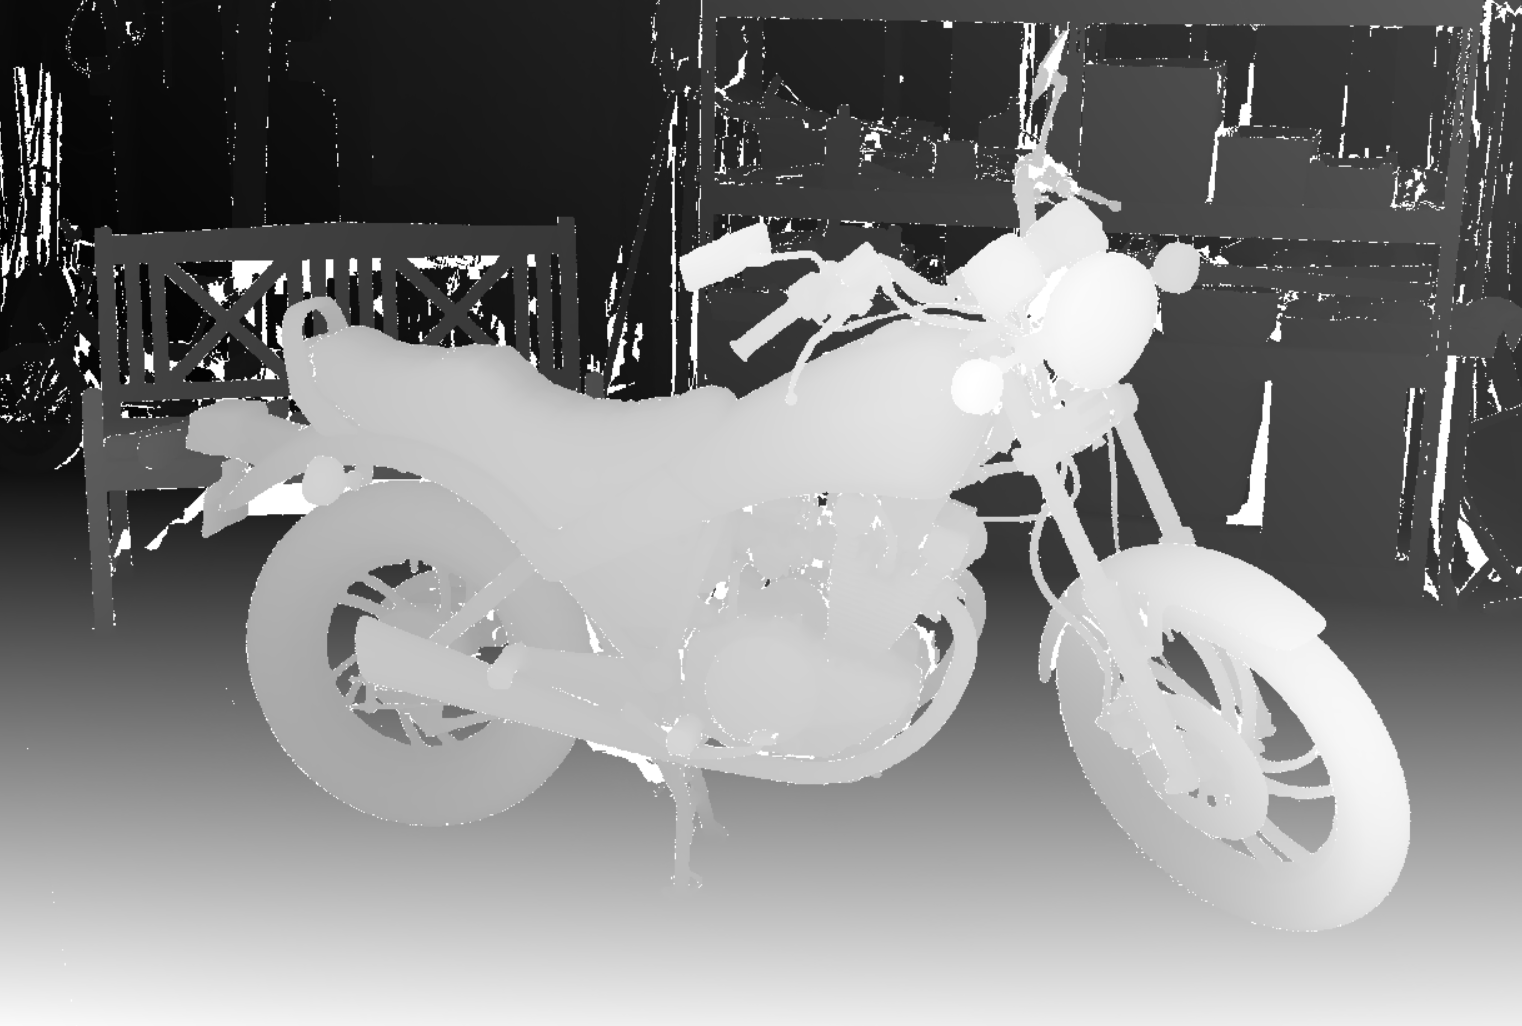
\includegraphics[width=0.4\textwidth]{images/im-0-disp.png}
}
\caption{Middlebury 2014 dataset example}
\label{fig:dataset-example}
\end{figure}

In order to obtain accurate high-resolution stereo datasets, the authors of the described work based their idea on establishing ground-truth disparities from the input views.
In this manner, calibration problem are prevented and the process can be performed via structured light.
However, the drawback of this is that correct disparities can be achieved only for scene points that are non-occluded in both images.
Therefore, extending the idea in \cite{scharstein2003high}, that is based on a self-calibration of structured light sources from initial non-occluded disparities, they managed to register illumination disparities in half-occluded regions and model projector lens distortion as well. 
Moreover, imposing initial correspondences they enhance significantly the rectification accuracy.
Then, subpixel precision was obtained exploiting a high number of binary patterns under multiple exposures and applying a robust interpolation.\\
A brief overview of the pipeline of the process, deeply illustrated in \cite{Scharstein2014}, is now presented.\\

\begin{figure}[t]
	\begin{center}
		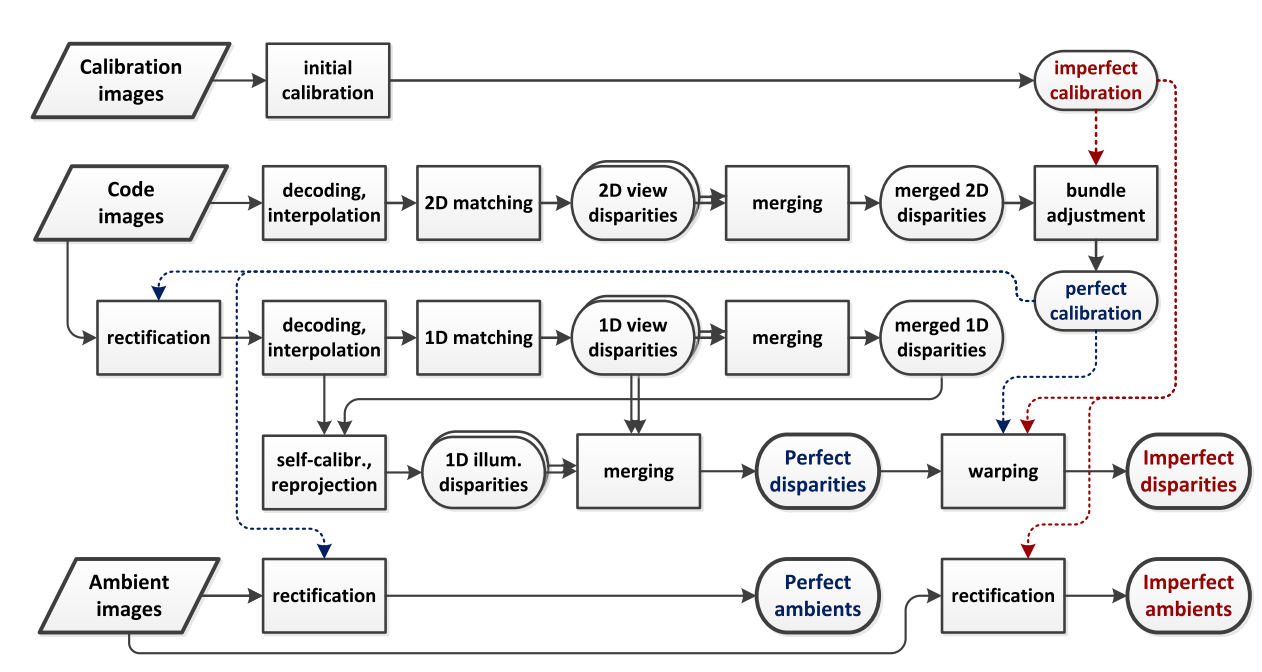
\includegraphics[width=.8\textwidth]{images/middlebury-2014-pipeline.png}
		\caption{Pipeline of the overall system for creating the Middlebury 2014 dataset \cite{Scharstein2014}}
		\label{fig:middleury-pipeline}
	\end{center}
\end{figure}

Figure \ref{fig:middleury-pipeline} depicts the overall pipeline of the system defined by Scharstein et al. \cite{Scharstein2014} for reconstruct the stereo datasets.\\
As simply described, the system's inputs are: calibration images of a standard checker-board calibration target; code images obtained with structured lighting projectors from different positions; \textit{ambient} images collected with multiple lighting conditions. 
First of all, re-factoring operations are applied to the unrectified code images, i.e. thresholding, decoding and interpolation.
This leads to floating-point coordinates of the projector pixel illuminating the scene. 
Thus, the achieved values are employed as unique identifiers to impose the correspondences between the two input images. 
So that, the resulting \textit{2D view disparities} are used to refine the \textit{imperfect} calibration in the bundle-adjustment phase.
The next step of the process is use the rectified input images to generate the \textit{1D view disparity}.
The self-calibration of the projector is, therefore, accessed using the merged disparities and thereby produce the \textit{1D illumination disparities}.
View and illumination disparities are, then, combined together into the \textit{perfect} disparities. 
Last row in Figure \ref{fig:middleury-pipeline} shows that rectifying with both calibration allows to achieve the corresponding sets of ambient images.\\
Further details of the single steps of the process are reminded to the original paper \cite{Scharstein2014} so as not to make the discussion much convoluted.\\
Nevertheless, it is worth to disclose that considering the evaluation of the datasets showed in \cite{Scharstein2014}, the choice of the Middlebury 2014 images for the initial tests can be assumed as a correct decision.
As a matter of fact, experimental results reported in the original paper demonstrate how that datasets can be considered highly challenging in terms of accuracy and scene complexity.
Therefore, they can be assumed as a useful starting point for recovering information from the ground truth images available and for the stereo algorithm evaluation.\\



